\documentclass[12pt]{article}
\usepackage{preamble}

\pagestyle{fancy}
\fancyhead[LO,LE]{Математический анализ}
\fancyhead[CO,CE]{13.03.2024}
\fancyhead[RO,RE]{Лекции Далевской О. П.}


\begin{document}
    Для линейной параметризации форма дифференциала сохраняется

    $d^2 z = (\frac{\partial }{\partial x}dx + \frac{\partial}{\partial y}dy)^2 z \stackrel{\text{инвариант}}{=} z^{(n)}_t dt^n$

    Введем функцию: $z(x(t), y(t)) \stackrel{\text{обозн}}{=} \varphi (t)$ - $(n + 1)$ раз дифференцируема (композиция $(n + 1)$ дифференцируемых и линейных функций)

    Заметим, что $x = x_0 + \Delta x t \stackrel{t_0 = 0}{=} x_0$, $y = y_0 + \Delta y t \stackrel{t_0 = 0}{=} y_0$

    \[M \stackrel{t \to t_0 = 0}{\rightarrow} M_0\]

    То есть $z(M_0) = z(x_0, y_0) = z(x(t_0), y(t_0)) = \varphi (t_0) = \varphi(0)$

    Таким образом $\varphi(t)$ как функция одной переменной может быть разложена в окрестности $t_0 = 0$ по формуле Маклорена

    \[\varphi(t) = \varphi(0) + \frac{d\varphi(0)}{1!} \Delta t + \dots + \frac{d^{n}\varphi(0)}{n!} \Delta t^n + o((\Delta t)^n)\]

    Вернемся к $z(x, y)$ ($\Delta t = t - t_0 = 1$):

    \[z(x, y) = z(M) = z(M_0) + \frac{dz(M_0)}{1!} + \frac{d^2 z(M_0)}{2!} + \dots + \frac{d^n z(M_0)}{n!} + r_n(x, y)\]

    где $r_n(x, y) = r_n(t) \stackrel{\text{Лагр.}}{=} \frac{\varphi^{(n+1)}(\theta \Delta t)}{(n + 1)!} \Delta t = \frac{\varphi^{(n+1)}(\theta \Delta t)}{(n + 1)!}$

    $r_n(x, y)$ должен быть б. м. по отношению к $(\Delta \rho)^n$, то есть $r_n(x, y) = o((\Delta \rho)^n)$

    ($r_n(t) \stackrel{n \to \infty}{\rightarrow}$, если $\varphi(t)$ нужное число раз дифференцируема $Rightarrow$ ограничена, $r_n(t)$ - огр. б. м.)

    \Nota В дальнейшем для исследования $z(x, y)$ на экстремум достаточно разложения по формуле Тейлора до 2-ого порядка включительно.
    Покажем сходимость $r_n(x, y) \stackrel{(\Delta \rho)^n \to 0}{\rightarrow} 0$ на примере $\displaystyle r_2 (x, y) = \frac{d^3 z(M_{\text{сред.}})}{3!}$


    $r_2(x, y) = \frac{1}{3!} (\frac{\partial}{\partial x} \Delta x + \frac{\partial}{\partial y} \Delta y)^3 z =
    \frac{1}{3!} (\frac{\partial^3 z}{\partial x^3} (\Delta x)^3 + 3 \frac{\partial^3 z}{\partial x^2 \partial y} (\Delta x)^2 \Delta y +
    3 \frac{\partial^3 z}{\partial x \partial y^2} (\Delta y)^2 \Delta x \frac{\partial^3 z}{\partial y^3} (\Delta y)^3)$

    Вообще говоря, значения частных производных берутся в различных средних точках

    $r_2(x, y) = \frac{1}{3!} (z_{xxx}(\mu_1)(\Delta x)^3 + 3 z_{xxy}(\mu_2)(\Delta x)^2 \Delta y + z_{xyy}(\mu_3)(\Delta y)^2 \Delta x + 3 z_{yyy}(\mu_4)(\Delta y)^3) = \Big|$ вынесем $(\Delta \rho)^3$

    $= \frac{(\Delta \rho)^3}{3!} (\text{огран.} \cdot \frac{(\Delta x)^3}{(\Delta \rho)^3} + \text{огран.} \cdot \frac{(\Delta x)^2 \Delta y}{(\Delta \rho)^3} + \text{огран.} \cdot \frac{(\Delta y)^2 \Delta x}{(\Delta \rho)^3} + \text{огран.} \cdot \frac{(\Delta y)^3}{(\Delta \rho)^3})$

    $\frac{(\Delta x)^3}{(\Delta \rho)^3} = \frac{(\Delta x)^3}{\sqrt{(\Delta x)^2 + (\Delta y)^2}^3} \stackrel{\Delta x \to 0}{\rightarrow} 0$, то есть дробь и выражение выше ограничены

    $\frac{r_2(x, y)}{(\Delta \rho)^2} = \frac{1}{3!} \frac{(\Delta \rho)^3 \cdot \text{огр.}}{(\Delta \rho)^2} = \frac{1}{3!} \Delta \rho \cdot \text{огр.} \stackrel{\Delta \rho \to 0}{\rightarrow} 0$

    \section{4.7. Геометрия ФНП}


    \section{4.7.1. Линии и поверхности уровня}

    Положим $z = const$. В сечении плоскостью $z = c$ образуется кривая $l$ с уравнением $\begin{cases}z = c \\ \varphi(x, y) = 0 \leftarrow \text{уравнение $l_\text{проек}$ на $Oxy$}\end{cases}$

    Кривая $l$ с уравнением $z(x, y) = c$ называется линией уровня Ф$_2$П $z = z(x, y)$

    \Def Поверхность уровня $\mathcal{P}$ - это поверхность с уровнем $u(x, y, z) = c$

    Физ. смысл: Пусть $u : \Real^3 \rightarrow \Real$ (значения функции $u(x, y, z)$ - скаляры). Тогда говорят, что в $\Real^3$ задано скалярное поле. Например, поле температур, давления, плотности и т. д.

    Тогда $u = c$ - поверхности постоянных температур, давления и т. п. (изотермические, изобарные, эквипотенциальные)

    \Ex Конус - $z = -\sqrt{x^2 + y^2}$

    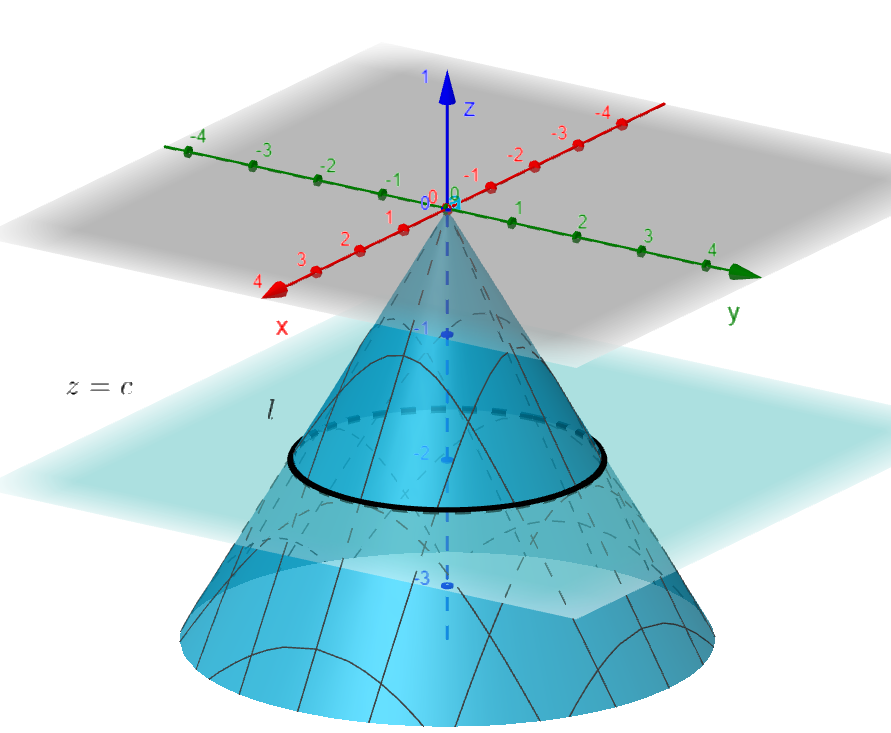
\includegraphics[height=90mm]{images/calculus_2024_03_13_1}

    Линии уровня $z = c$:

    \begin{enumerate}
        \item $c > 0 \quad \emptyset$
        \item $c = 0 \quad x = y = 0 - $ точка $(0, 0)$
        \item $c < 0 \quad -|c| = -\sqrt{x^2 + y^2} \quad c^2 = x^2 + y^2$
    \end{enumerate}


    \section{4.7.2. Производная по направлению, Градиент}

    Задача. Дано скалярное поле $u = u(x, y, z)$ (напр. давления). Как меняется давление при перемещении в заданном направлении?

    Это задача о нахождении скорости изменения $u(x, y, z)$ в заданном направлении $\overrightarrow{s}$

    Из $M_0(x_0, y_0, z_0)$ движемся в $M(x, y, z)$ в направлении $\overrightarrow{s}$, $x = x_0 + \Delta x$, $y = y_0 + \Delta y$, $z = z_0 + \Delta z$

    $\Delta s = \sqrt{(\Delta x)^2 + (\Delta y)^2 + (\Delta z)^2} \quad \Big| \cdot \frac{1}{\Delta s}$

    $1 = \sqrt{(\frac{\Delta x}{\Delta s})^2 + (\frac{\Delta y}{\Delta s})^2 + (\frac{\Delta z}{\Delta s})^2}$

    $(\frac{\Delta x}{\Delta s}, \frac{\Delta y}{\Delta s}, \frac{\Delta z}{\Delta s}) = (\cos\alpha, \cos\beta, \cos\gamma) = \overrightarrow{s^0}$

    Потребуем, чтобы $u(x, y, z)$ имела непрерывность $u_x, u_y, u_z$ в $D$

    То есть $u(x, y, z)$ дифференцируема и

    $\Delta u = du + o(\Delta s) = u_x \Delta x + u_y \Delta y + u_z \Delta x + o(\Delta s) \quad \Big| \cdot \frac{1}{\Delta s}$

    $\frac{\Delta u}{\Delta s} = u_x \cos\alpha + u_y \cos\beta + u_z \cos\gamma + \frac{o(\Delta s)}{\Delta s}$ - предельный переход

    $\frac{\partial u}{\partial s} = \frac{\partial u}{\partial x} \cos\alpha + \frac{\partial u}{\partial y} \cos\beta + \frac{\partial u}{\partial z} \cos\gamma$

    \Nota Изначально $\Delta u = du + \text{(б. м.)} \Delta x + \text{(б. м.)} \Delta y + \text{(б. м.)} \Delta z \quad \Big| \cdot \frac{1}{\Delta s}$

    $\frac{\Delta u}{\Delta s} = \frac{du}{\Delta s} + \text{(б. м.)} \cos\alpha$, $\text{(б. м.)} \cos\alpha \rightarrow 0$

    \Def $\frac{\partial u}{\partial s} = \frac{\partial u}{\partial x} \cos\alpha + \frac{\partial u}{\partial y} \cos\beta + \frac{\partial u}{\partial z} \cos\gamma$

    где $\alpha, \beta, \gamma$ - направления $\overrightarrow{s}$, называют производной функции $u = u(x, y, z)$ в направлении $\overrightarrow{s}$

    \Nota Производная в определении - число, но $\frac{\partial u}{\partial s} \overrightarrow{s^0}$ - вектор скорости

    \Nota Заметим, что если $\overrightarrow{i}, \overrightarrow{j}, \overrightarrow{k}$ - декартовы орты, то

    $\frac{\partial u}{\partial i} = \frac{\partial u}{\partial x} 1 + \frac{\partial u}{\partial y} 0 + \frac{\partial u}{\partial z} 0 = \frac{\partial u}{\partial x}$

    и аналогично в других направлениях: $\frac{\partial u}{\partial j} = \frac{\partial u}{\partial y}, \frac{\partial u}{\partial k} = \frac{\partial u}{\partial z}$

    Составим вектор $\frac{\partial u}{\partial x} \overrightarrow{i} + \frac{\partial u}{\partial y} \overrightarrow{j} + \frac{\partial u}{\partial z} \overrightarrow{k} \stackrel{\text{обозн}}{=} \overrightarrow{\triangledown} u$

    $\overrightarrow{\triangledown}$ - набла-оператор (оператор Гамильтона); $\overrightarrow{\triangledown} = (\frac{\partial}{\partial x}; \frac{\partial}{\partial y}; \frac{\partial}{\partial z})$ - условный вектор

    \Def $\overrightarrow{grad} \ u \stackrel{def}{=} \overrightarrow{\triangledown} u$ - называют градиентом функции $u(x, y, z)$

    Свойства градиентов:

    \ThN{1} $\frac{\partial u}{\partial s} = \text{пр.}_{\overrightarrow{s}} \overrightarrow{\triangledown} u$

    \ThN{2} $\overrightarrow{\triangledown} u$ - направление наибольшего значения $\frac{\partial u}{\partial s}$

    \ThN{3} $\overrightarrow{s} \perp \overrightarrow{\triangledown} u \Longrightarrow \frac{\partial u}{\partial s} = 0$

    \ThN{4} $u = u(x, y), u = c$ - линии уровня $l$. Тогда $\overrightarrow{\triangledown} u \perp l$

    Доказательства:

    \begin{enumerate}
        \item $\frac{\partial u}{\partial s} = (\frac{\partial}{\partial x}; \frac{\partial}{\partial y}; \frac{\partial}{\partial z}) \cdot \overrightarrow{s^0} =
        \overrightarrow{\triangledown} u \overrightarrow{s^0} = |\overrightarrow{\triangledown} u| |\overrightarrow{s^0}| \cos(\overrightarrow{\triangledown} u, \overrightarrow{s^0}) =
        |\overrightarrow{\triangledown} u| \cos(\overrightarrow{\triangledown} u, \overrightarrow{s^0}) = \text{пр.}_{\overrightarrow{s}} \overrightarrow{\triangledown} u$

        \item $\frac{\partial u}{\partial s} = |\overrightarrow{\triangledown} u| \cos\varphi \dots $ \Lab

        \item \Lab

        \item $u = c$ - уравнение $l_{\text{пр}}$ в плоскости $Oxy$, то есть $u(x, y) = c$, можем рассмотреть как неявную функцию $u(x, y(x)) - c = 0$

        Производная неявной функции: $\frac{dy}{dx} = -\frac{u_x}{u_y} = k_l$ - угловой коэффициент касательной к $l$

        $\overrightarrow{\triangledown} u = (u_x, u_y) \quad \frac{u_y}{u_x} = k_{\text{град.}}$ - наклон вектора градиента.
        Очевидно $k_l \cdot k_{\text{град.}} = -1 \Longrightarrow \overrightarrow{\triangledown} u \perp l$
    \end{enumerate}



\end{document}
